\documentclass[xcolor=pdftex,hyperref={pdfpagelabels=false},table,10pt]{beamer}

\definecolor{fudepan}{HTML}{006c63}
\definecolor{verde}{RGB}{0, 127, 63}
\definecolor{gris}{RGB}{86, 86, 86}
\definecolor{listinggray}{gray}{0.9}
\definecolor{lbcolor}{rgb}{0.95,0.95,0.95}

\usetheme{Warsaw}
\usecolortheme[named=verde]{structure}

% \setbeamercolor{frametitle}{bg=black}
% \setbeamercolor{frametitle right}{bg=verde}

\usefonttheme{structurebold}
\useinnertheme{rounded}
\setbeamercovered{transparent}

\usepackage[spanish]{babel}
\usepackage[utf8]{inputenc}
\usepackage{listings}

\defbeamertemplate*{footline}{shadow theme}
{%
  \leavevmode%
  \hbox{\begin{beamercolorbox}[wd=.5\paperwidth,ht=2.5ex,dp=1.125ex,leftskip=.3cm plus1fil,rightskip=.3cm]{author in head/foot}%
    \usebeamerfont{author in head/foot}\insertframenumber\,/\,\inserttotalframenumber\hfill\insertshortauthor
  \end{beamercolorbox}%
  \begin{beamercolorbox}[wd=.5\paperwidth,ht=2.5ex,dp=1.125ex,leftskip=.3cm,rightskip=.3cm plus1fil]{title in head/foot}%
    \usebeamerfont{title in head/foot}\insertshorttitle:\ Abstracción de distribución de procesos recursivos
  \end{beamercolorbox}}%
  \vskip0pt%
}

\lstset{
    backgroundcolor=\color{lbcolor},
    tabsize=4,6
    rulecolor=,
    language=matlab,
        basicstyle=\scriptsize,
        upquote=true,
        aboveskip={1.5\baselineskip},
        columns=fixed,
        showstringspaces=false,
        extendedchars=true,
        breaklines=true,
        prebreak = \raisebox{0ex}[0ex][0ex]{\ensuremath{\hookleftarrow}},
        frame=single,
        showtabs=false,
        showspaces=false,
        showstringspaces=false,
        identifierstyle=\ttfamily,
        keywordstyle=\color[rgb]{0.1,0.1,0.6}\bfseries,
        commentstyle=\color[rgb]{0.133,0.545,0.133},
        stringstyle=\color[rgb]{0.627,0.126,0.941},
}

\title{RecAbs}
\subtitle{Abstracción de distribución de procesos recursivos implementada sobre FuD}
\author{Mariano Bessone \& Emanuel Bringas}
\institute[UNRC]{
    
    %Escudos
    \begin{minipage}{0.45\textwidth}
        \begin{center}
            %Escudo UNRC
            
\includegraphics[scale=0.23]{images/unrc.jpg}\\
            \begin{scriptsize}
                \textsc{Universidad Nacional de Río Cuarto} \\
            \end{scriptsize}
            \vfill
            \begin{tiny}
                \textsc{Fac. de Cs. Exactas, Fco-Qcas y Naturales} \\
                \textsc{Departamento de Computación} \\[1cm]
            \end{tiny}
        \end{center}
    \end{minipage}
    \begin{minipage}{0.45\textwidth}
        \begin{center}
            %Escudo FuDePAN
            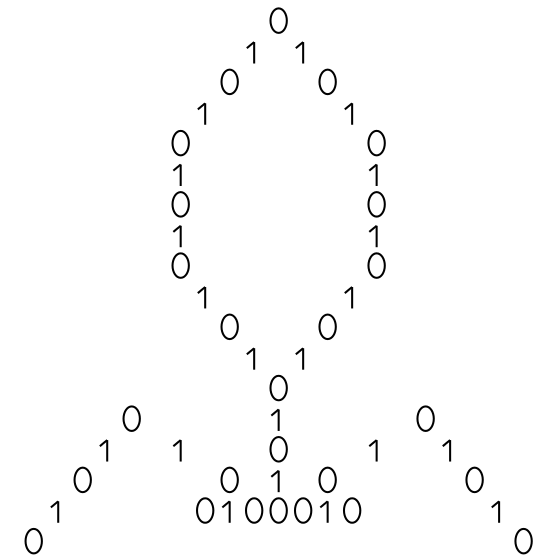
\includegraphics[scale=0.1]{images/fudepan.png}\\
            \vfill
            \begin{scriptsize}
                \textsc{FuDePAN} \\
            \end{scriptsize}
            \begin{tiny}
                \textsc{Fundación para el Desarrollo de la Programación en Ácidos Nucleicos} \\[1cm]
            \end{tiny}
        \end{center}
    \end{minipage}
}
\date{19 de Diciembre de 2011}

\newcommand{\fude}{\textbf{FuDePAN}}
\newcommand{\rc}{\textbf{RecAbs}}
\newcommand{\fud}{\textbf{FuD}}
\newcommand{\combeng}{\textbf{CombEng}}
\newcommand{\rnaffe}{\textbf{RnaFFE}}
\newcommand{\cpp}{\textbf{C++}}

\begin{document}

\begin{frame}
    \titlepage
\end{frame}


\begin{frame}
    \frametitle{Temario}
    \tableofcontents
\end{frame}

\chapter{Introducción}

La idea original de este proyecto nace de \fude{} (\textbf{Fu}ndación para el \textbf{De}sarrollo de la \textbf{P}rogramación en
\textbf{Á}cidos \textbf{N}ucleicos), organización sin fines de lucro que se dedica a la investigación y desarrollo en bioinformática,
aplicándola a problemas biológicos asociados a la salud humana. En esta fundación se utiliza a la computación para hacer simulaciones y
cálculos para, por ejemplo, mejorar vacunas, mejorar tratamientos contra enfermedades como el HIV, o el virus Junín, desarrollando y
utilizando herramientas informáticas y programación de avanzada.\\

La mayoría de los problemas que la fundación enfrenta diariamente son de gran complejidad, por lo que se requiere de altos recursos
computacionales para lograr tener resultados a corto plazo. Es por ello que existe el framework \fud\cite{clus09} para la distribución
automática de trabajos en nodos de cómputo, que permite mediante una simple reimplementación de proyectos ya desarrollados de manera
secuencial, obtener una versión paralelizada del mismo. De esta manera se logró obtener resultados confiables en un tiempo relativamente
corto.\\

Asimismo, se notó que muchos problemas bioinformáticos, corrientes y a futuro, son naturalmente solucionados usando recursión pero no había
una forma de agruparlos y facilitar su desarrollo. Por esta razón, surge la motivación de construir una implementación genérica a toda
solución recursiva como una capa más del framework.\\

Los objetivos planteados al comienzo del proyecto fueron los siguientes:
\begin{itemize}
    \item   Diseñar una abstracción que permita a cualquier programador de la fundación poder construir soluciones recursivas paralelizadas
            de una manera sencilla. Evitando así la dificultad que conlleva lidiar con problemas inherentes a la programación paralela.
    \item   Construir esta abstracción como una aplicación particular de \fud{} que abarque toda solución recursiva de un problema que no
            requiera \textit{backtracking}.
    \item   Refactorizar \fud{} con el fin de aportar funcionalidades de interactividad entre cliente y servidor, lo cuál es necesario para
            el desarrollo de \rc. Este rediseño debe respetar los principios originales del framework, para que toda aplicación que lo use
            lo siga haciendo sin modificación alguna en la nueva versión.
    \item   En ambas implementaciones procurar cumplir con los requisitos de calidad y performance en cuánto a código y diseño.
\end{itemize}

Este documento proporciona una visión general sobre el diseño y detalles de implementación de los puntos mencionados anteriormente, junto
con ejemplos de su uso y algunos resultados estadísticos sobre el rendimiento de aplicaciones.\\

El informe se divide en 4 partes. La Parte \ref{part:prelim} incluye una introducción a este trabajo, un capítulo con el marco teórico para
facilitar la lectura de este documento y otro con la metodología de trabajo utilizada para llevar a cabo el proyecto.

La Parte \ref{part:recabs} contiene todo lo relacionado con \rc, a partir del enunciado del problema y el enfoque de la solución tomado, el
lector encontrará detalles acerca del diseño e implementación de la capa, junto con ejemplos sencillos de su uso.

La Parte \ref{part:refactorin_fud} introduce el problema de montado \rc/\fud, seguido de la refactorización del framework, con el fin de
acoplar la capa de abstracción de distribución de procesos recursivos sobre éste.

Finalmente, la Parte \ref{part:conclusion} brinda la conclusión sobre la tesis y un mapa de los trabajos que quedan por hacer.

En la parte de apéndices, hay dos reportes de métricas de código generados automáticamente, tanto de \rc{} como de la refactorización de
\fud, y documentación sobre patrones de diseño utilizados en este proyecto.

\section{RecAbs}

\begin{frame}\frametitle{¿Qué es \rc?}
    \begin{itemize}
        \item   Abstracción genérica para soluciones recursivas.
                % Definición, problemas que ataca.
        \item   Arquitectura cliente-servidor.
                % Se creo con esta arquitectura para el posible montado con cualquier middleware de distribución.
        \item   Técnica de descomposición de datos recursiva.
                % Ciencia: principio de diseño de algoritmos paralelos.
        \pause
        \item   Se optó por implementarla como una nueva capa de \fud{}.
    \end{itemize}

    \begin{center}
        \only<1>{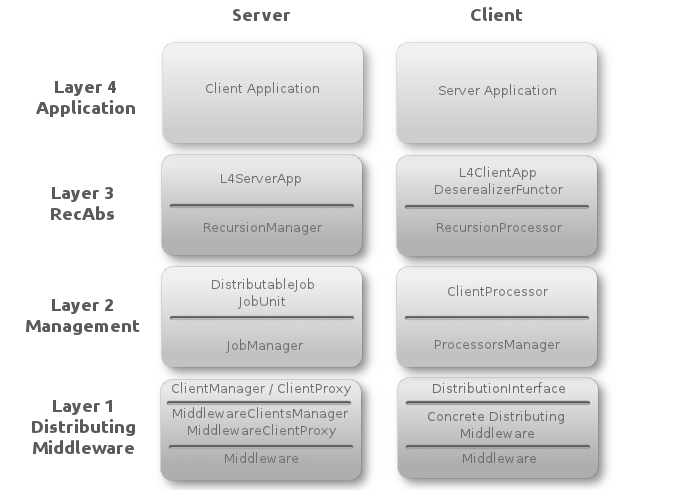
\includegraphics[scale=.29]{images/recabs1.png}}
        \only<2>{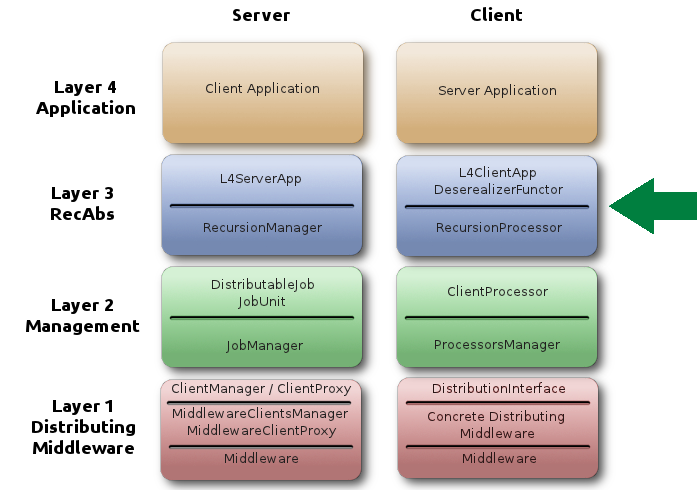
\includegraphics[scale=.29]{images/recabs2.png}}
    \end{center}
\end{frame}


\begin{subsection}{Diseño}

\begin{frame}{Principios de Diseño}

    \begin{block}{Evitar}
        \begin{itemize}
            \item \textbf{Rigidez}: es difícil modificar porque cada cambio afecta a muchas otras partes del sistema.
            \item \textbf{Fragilidad}: cuando hacemos un cambio, partes inesperadas del sistema se rompen.
            \item \textbf{Inmovilidad}: es difícil reutilizar componentes en otra aplicación, ya que no se pueden desligar de la       
                aplicación actual.
        \end{itemize}
    \end{block}

    \begin{block}{Principios \textbf{SOLID}}
        \begin{itemize}
            \item   \textbf{S}ingle Responsibility Principle (SRP)
            \item   \textbf{O}pen-Closed Principle (OCP)
            \item   \textbf{L}iskov Substitution Principle (LSP)
            \item   \textbf{I}nterface Segregation Principle (ISP)
            \item   \textbf{D}ependency Inversion Principle (DIP)
        \end{itemize}
    \end{block}
\end{frame}

\begin{frame}\frametitle{Diagrama de Clases}
    \begin{center}
        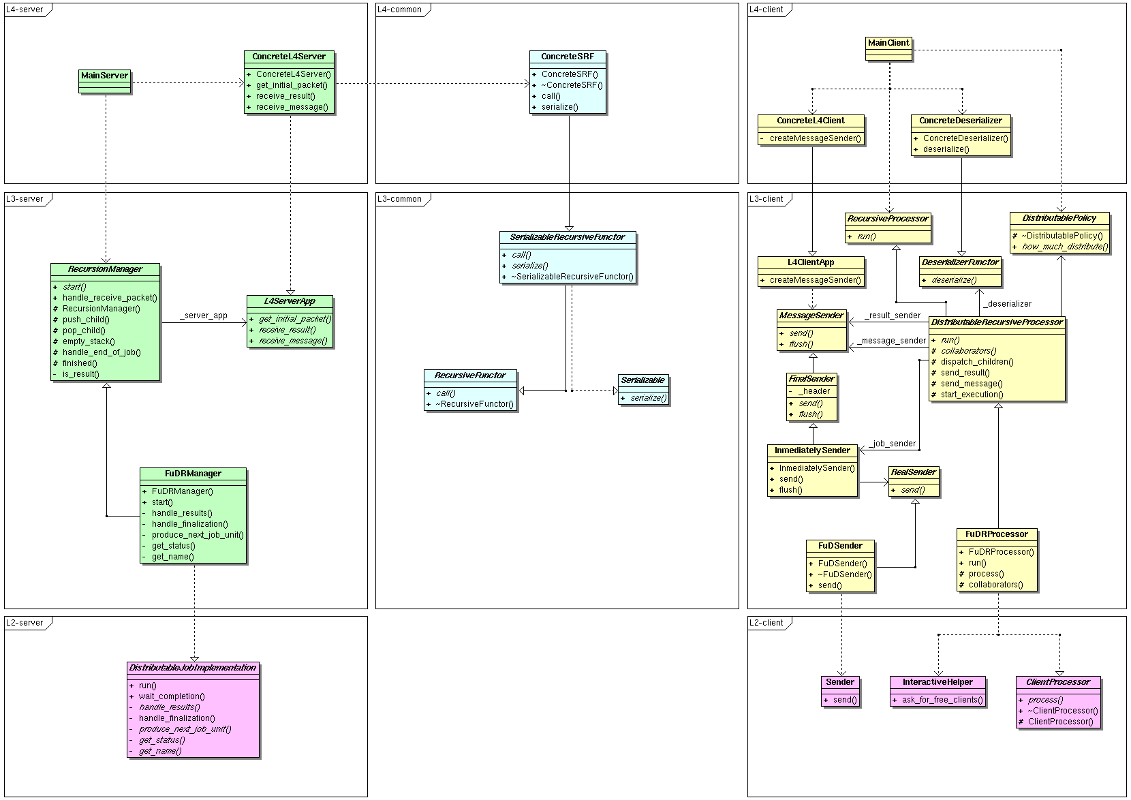
\includegraphics[scale=0.25]{images/class.png}
    \end{center}
\end{frame}


\begin{frame}\frametitle{Lado Común}
    \begin{center}
        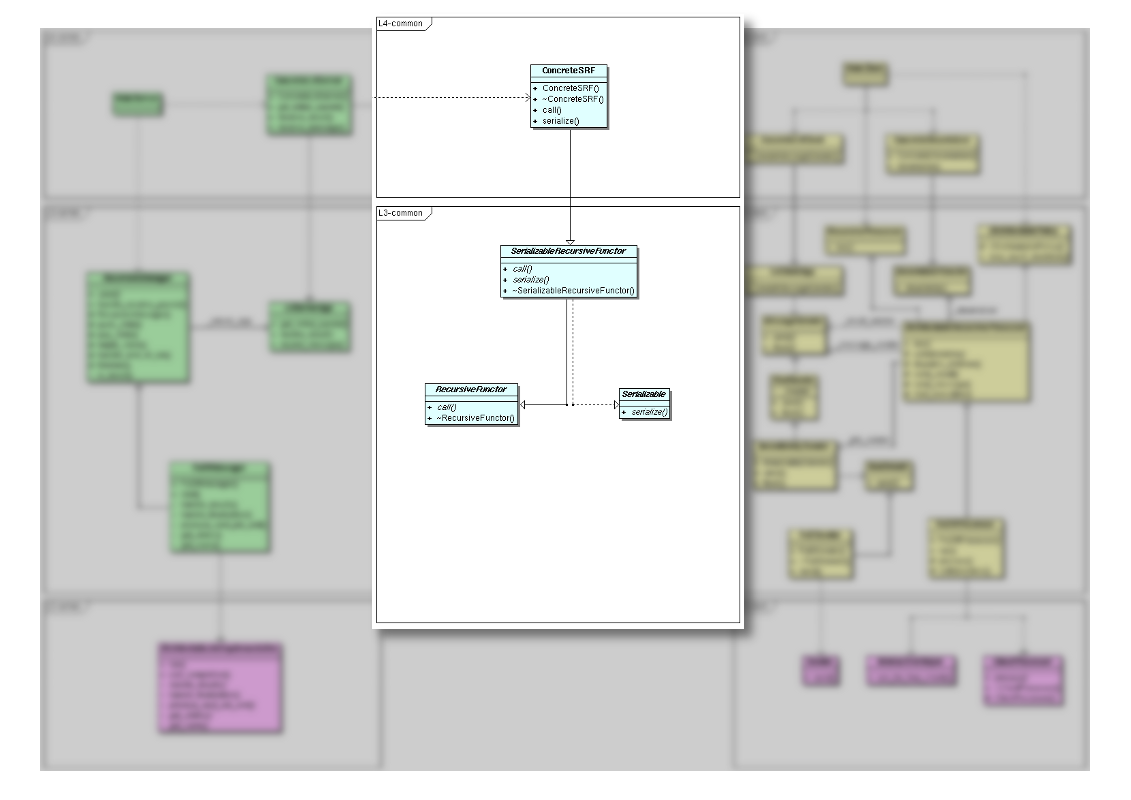
\includegraphics[scale=0.25]{images/class-common-side.png}
    \end{center}
\end{frame}

\begin{frame}\frametitle{Lado Común: Functor Recursivo}% Functor Recursivo
    \textbf{Functor Recursivo}
    \begin{itemize}
     \item Abstracción que representa una función recursiva
     \item Describe un estado particular de la función
     \item Especifica de cada aplicación
     \item Implementa su serialización.
    \end{itemize}

    \begin{center}
        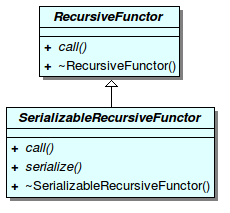
\includegraphics[scale=0.4]{images/srf.png}
    \end{center}
    
\end{frame}



\begin{frame}\frametitle{Lado Servidor}
    \begin{center}
        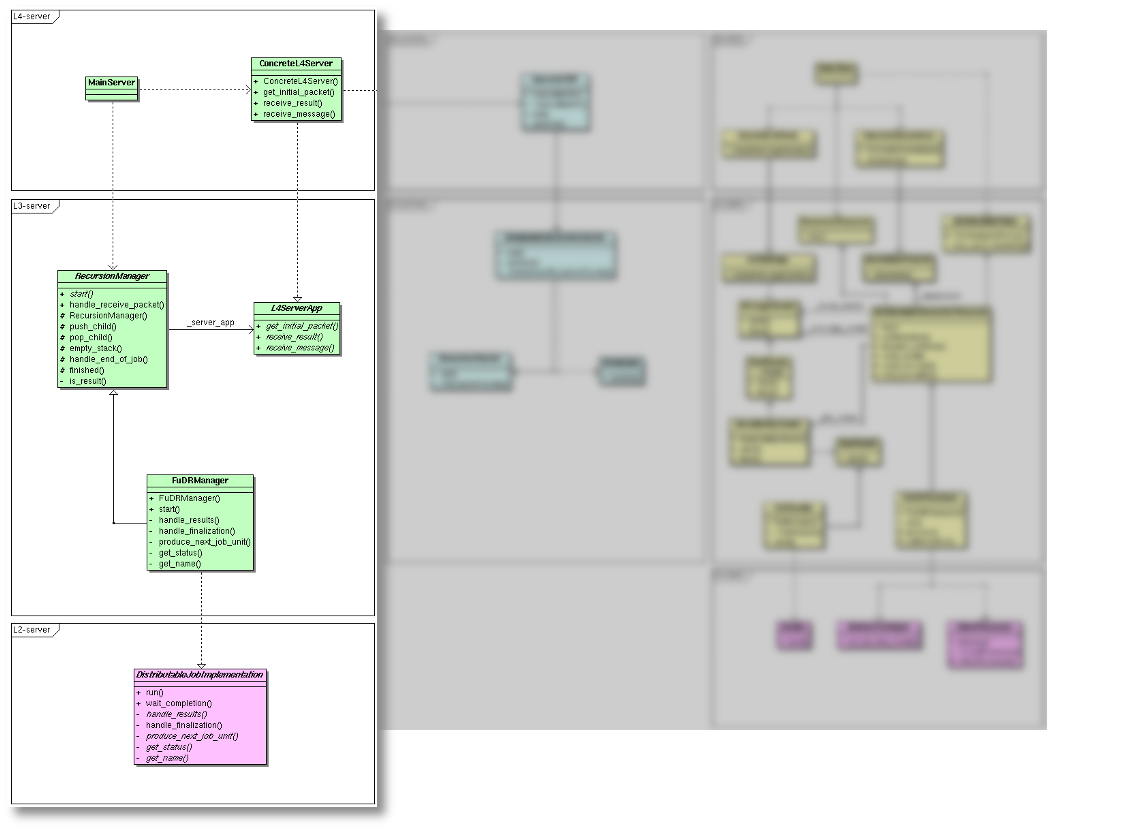
\includegraphics[scale=0.25]{images/class-server-side.png}
    \end{center}
\end{frame}

\begin{frame}\frametitle{Lado Servidor: Asistente del Servidor}% Asistente del Servidor

    \textbf{Asistente del Servidor}

    Especifica detalles de como iniciar el procesamiento y manipular mensajes.

    \begin{block}{Responsabilidades}
        \begin{itemize}
            \item   Brindar el \textit{functor} inicial
            \item   Definir que hará con los resultados a medida que lleguen
            \item   Definir el tratamiento de los mensajes intermedios %(si es que los hubiera).
        \end{itemize}
    \end{block}

    \begin{center}
        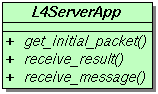
\includegraphics[scale=0.4]{images/l4_server_app.png}
    \end{center}

% De estos requisitos, el primero es obligatorio y los dos restantes son opcionales en la medida de que la aplicación arroje resultados
% y mensajes intermedios.
\end{frame}

\begin{frame}\frametitle{Lado Servidor: Administrador de la Recursión}% Administrador de la Recursión

    \textbf{Administrador de la Recursión}  

    \begin{itemize}
     \item Inicia la ejecución
     \item Organiza y manipula los functores pendientes
     \item Interactúa con le middleware de distribución
    \end{itemize}

     \begin{block}{Tipos de Mensajes}
        \begin{itemize}
            \item  \textbf{Resultado}, parcial y relativo a la unidad de trabajo que se procesó
            \item  \textbf{Mensaje Intermedio} es cualquier dato transmitido de cliente a servidor sin llegar a una hoja o
                    estado final en el árbol
            \item  \textbf{Unidad de Trabajo} functor intermedio a distribuir, la cuál será enviada a un cliente ocioso. Un \textit{trabajo}
                arribado es una partición del trabajo del cliente que lo envió.
        \end{itemize}
     \end{block}


\end{frame}

\begin{frame}\frametitle{Lado Servidor: Administrador de la Recursión}% Administrador de la Recursión (Diagrama de Clases) 

    \begin{center}
       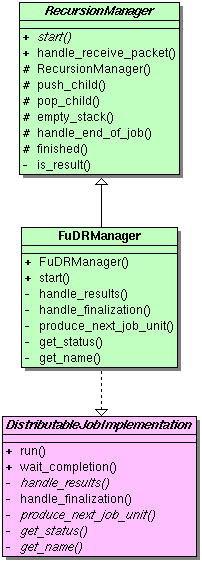
\includegraphics[scale=0.3]{images/fud_manager_dji.png}
    \end{center}

\end{frame}



\begin{frame}\frametitle{Lado Cliente}
    \begin{center}
        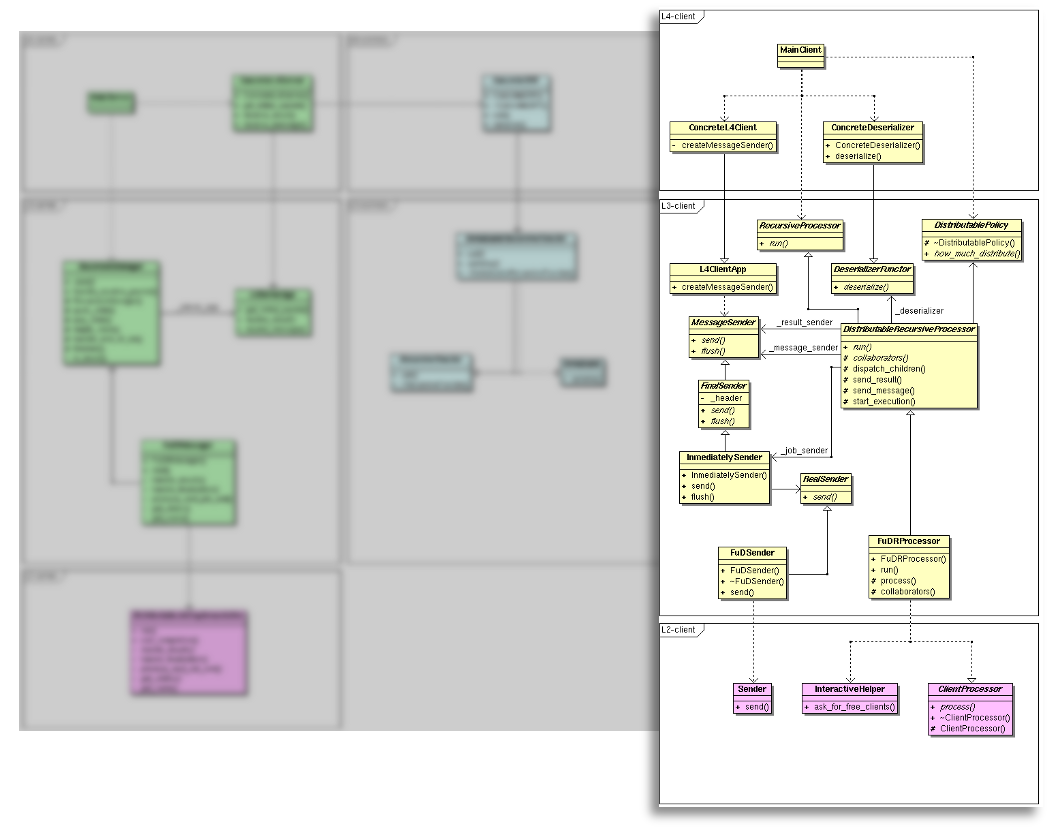
\includegraphics[scale=0.25]{images/class-client-side.png}
    \end{center}
\end{frame}

\begin{frame}\frametitle{Lado Cliente: Procesador Recursivo} %Procesador Recursivo
    \textbf{Procesador Recursivo}
    
    Engine de ejecución recursiva, se encarga de llevar a cabo el procesamiento total de un functor en un nodo.

    \begin{block}{Responsabilidades}
        \begin{itemize}
        \item Administra la reproducción de functores hijos
        \item Analizar y efectuar la redistribucion de los mismos
        \item Permitir el envío de mensajes y resultados al servidor
        \item Recolecta functores en caso base y los envía al servidor
        \end{itemize}
    \end{block}
\end{frame}

\begin{frame}\frametitle{Lado Cliente: Procesador Recursivo} %Procesador Recursivo, Diagrama de clases
    \begin{center}
         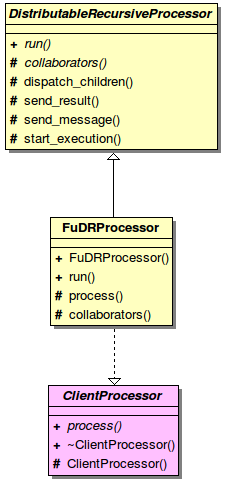
\includegraphics[scale=0.4]{images/frp.png}
    \end{center}
\end{frame}

\begin{frame}\frametitle{Lado Cliente: Senders}
    \textbf{Senders}

    \begin{itemize}
        \item Manipulan los mensajes a enviar
        \item Interactúa con el middleware de distribución
        \item Efectúan el envío
    \end{itemize}

    \begin{center}
     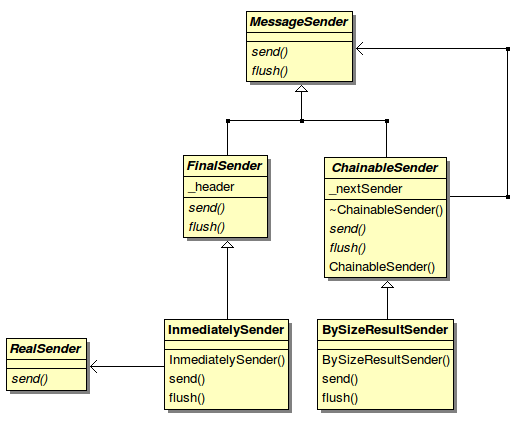
\includegraphics[scale=0.3]{images/senders.png}
    \end{center}
\end{frame}

\begin{frame}\frametitle{Lado Cliente: Asistente del Cliente y Deserializador}
    \textbf{Asistente del Cliente}

        Especifica el sender apropiado

    \begin{center}
        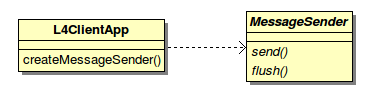
\includegraphics[scale=0.4]{images/l4_client_app.png}
    \end{center}

    \textbf{Deserializador}

    Especifica la manera en que se realiza el método inverso a la serialización realizada en el lado servidor

    \begin{center}
        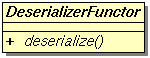
\includegraphics[scale=0.4]{images/deserializer.png}
    \end{center}        

\end{frame}

\begin{frame}\frametitle{Lado Cliente: Política de Distribución}

    \textbf{Política de distribución}
    Políticas que rigen el envío de trabajo pendiente al servidor con el fin de aprovechar la disponibilidad de clientes ociosos

    \pause
    \begin{block}{Establece}
        \begin{itemize}
            \item Cuando un cliente debe distribuir
            \item Cuanto trabajo debe distribuir
        \end{itemize}
    \end{block}

    \pause  
    Este tipo de políticas influye en la performance de una aplicación ya que el costo de comunicación varía dependiendo principalmente
    de:
    \begin{itemize}
        \item   Nivel de procesamiento que requiera la aplicación concreta
        \item   Recursos con que se cuenten (tanto en servidor como en clientes)
    \end{itemize}

\end{frame}

\begin{frame}\frametitle{Lado Cliente: Política de Distribución} %Diagrama de clases

    \begin{center}
        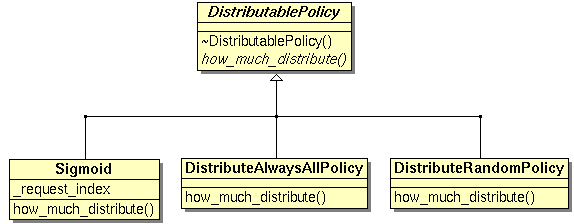
\includegraphics[scale=.25]{images/distribution_policy.png}
    \end{center}
    \pause
    \begin{center}
        $$fsd(x) = \frac{children-1}{1 + e^{-(\log_{children}{leafs}) * index + x - (children-1)}} $$
        \only<2>{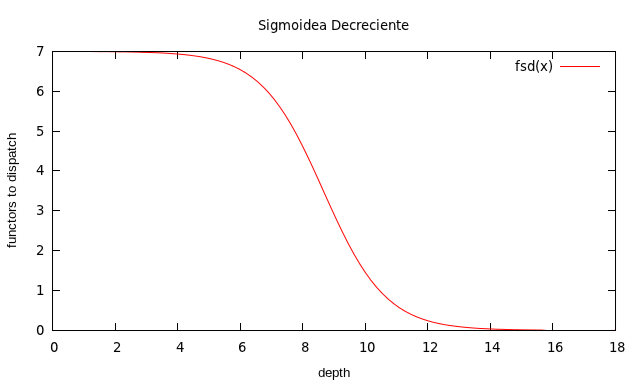
\includegraphics[scale=.25]{images/fsd.png}}
    \end{center}
\end{frame}



\end{subsection}

\subsection{Funcionamiento}

\begin{frame}\frametitle{¿Cómo funciona una aplicación \rc?}
    \begin{center}
        \only<1>{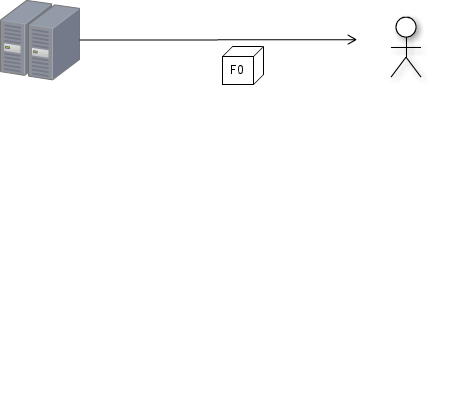
\includegraphics[scale=.45]{images/recabs_working_1.png}}
        \only<2>{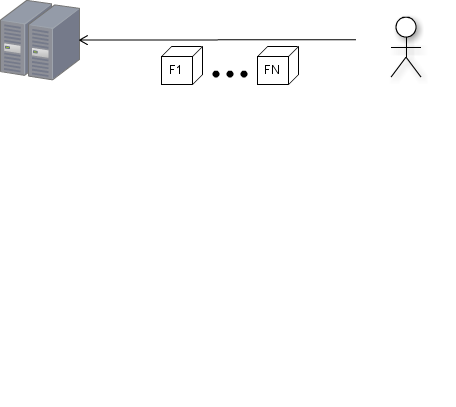
\includegraphics[scale=.45]{images/recabs_working_2.png}}
        \only<3>{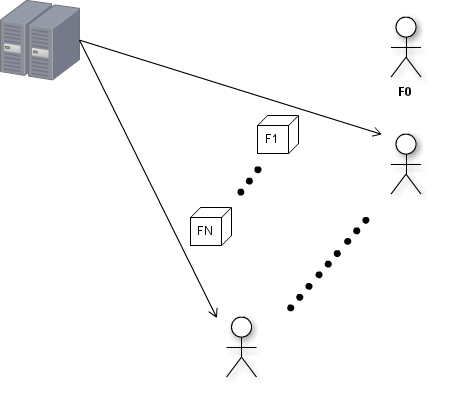
\includegraphics[scale=.45]{images/recabs_working_3.png}}
        \only<4>{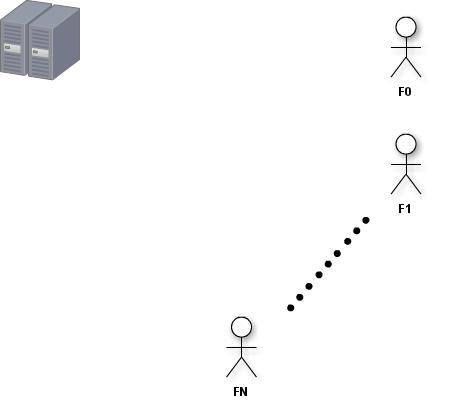
\includegraphics[scale=.45]{images/recabs_working_4.png}}
        \only<5>{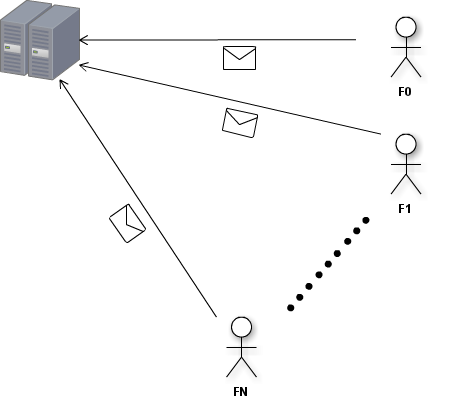
\includegraphics[scale=.45]{images/recabs_working_5.png}}
    \end{center}
\end{frame}

\begin{frame}
    \begin{columns}[T]
        \begin{column}{.3\textwidth}
            \begin{center}
                \textbf{SERVER}\\
                \textit{Inicio de recursión}
            \end{center}
        \end{column}
        \begin{column}{.7\textwidth}
            \centering
            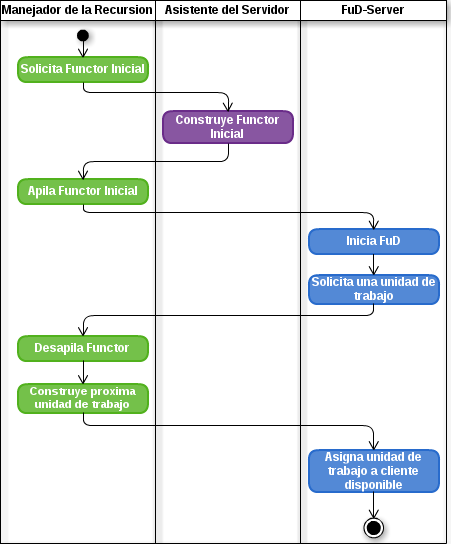
\includegraphics[scale=0.39]{images/ActivityRecAbs-1.png}
        \end{column}
    \end{columns}
\end{frame}

\begin{frame}
    \begin{columns}[T]
        \begin{column}{.3\textwidth}
            \begin{center}
                \textbf{CLIENTE}\\
                \textit{Procesamiento de functores}\\[1cm]
                \only<2>{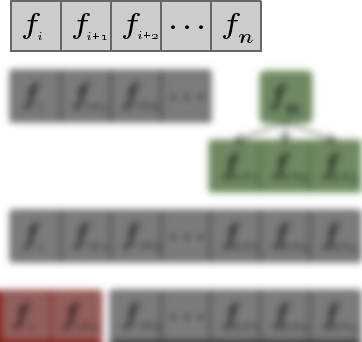
\includegraphics[scale=0.35]{images/DRP_Alg_1.png}}
                \only<3>{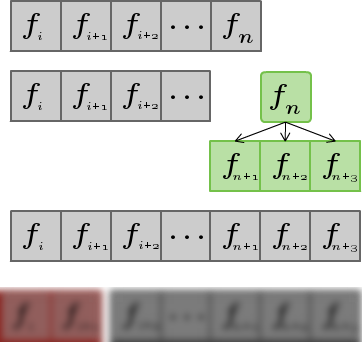
\includegraphics[scale=0.35]{images/DRP_Alg_2.png}}
                \only<4>{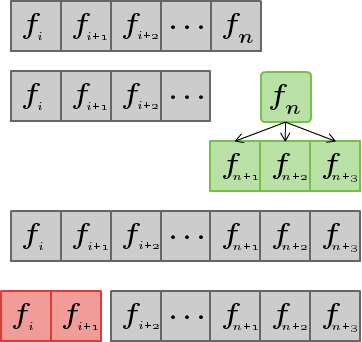
\includegraphics[scale=0.35]{images/DRP_Alg_3.png}}
            \end{center}
        \end{column}
        \begin{column}{.7\textwidth}
            \raggedleft
            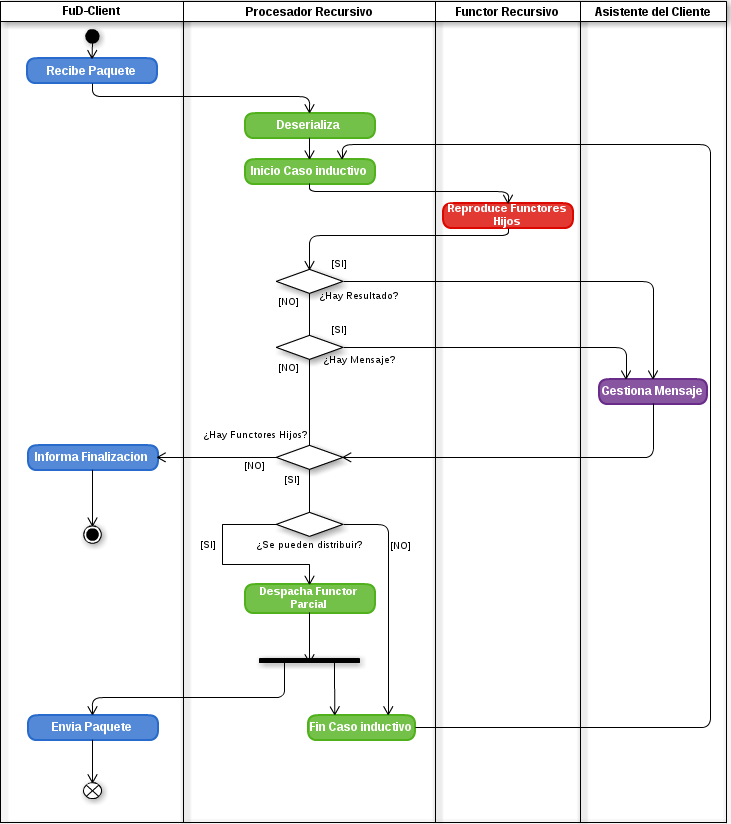
\includegraphics[scale=0.26]{images/ActivityRecAbs-2.png}
        \end{column}
    \end{columns}
\end{frame}

    \begin{frame}
    \begin{columns}[T]
        \begin{column}{.3\textwidth}
            \begin{center}
                \textbf{SERVER}\\
                \textit{Manejo de mensajes}
            \end{center}
        \end{column}
        \begin{column}{.7\textwidth}
            \centering
            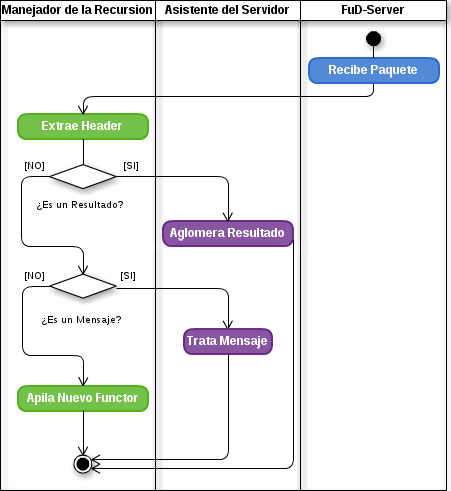
\includegraphics[scale=0.39]{images/ActivityRecAbs-3.png}
        \end{column}
    \end{columns}
\end{frame}


\subsection{Implementación}

\begin{frame}[fragile]\frametitle{Dependencias}

    \rc{} usa las siguientes librerías:
    \begin{description}
        \item[\fud]: framework de distribución elegido.
        \item[MiLi]: colección sencilla de pequeñas librerías útiles.
    \end{description}

    \lstset{language=C++}
    \begin{lstlisting}[frame=single]
/* The client sends a message. */
OutputMessage out;
out << _header << packet;
_real_sender->send(out);

/* The server receives the message. */
void handle_receive_packet(InputMessage& input)
{
    RecabsPacketHeader header;
    input >> header;
    switch(header)
    { ... }
}
    \end{lstlisting}
\end{frame}

\begin{frame}\frametitle{Métricas}
    \rc{} esta constituido por 23 archivos con un total de 2394 líneas de texto.

    \begin{center}
    \rowcolors{2}{verde!20}{verde!5}
    \begin{tabular}{|l|r|r|r|r|c|}
    \hline
    \multicolumn{2}{|c|}{Files} & \multicolumn{3}{|c|}{Line Types} & \hspace{0.2cm}\% \\
    \hline
    \textbf{Type} & \textbf{Count} & \textbf{Blank} & \textbf{Comment} & \textbf{Source} & \small{\textbf{\#Comms./Tot.}}\\
    \hline
    \texttt{C++ source} & 7   &    102  &     301   &    381 & 44.13 \\
    \hline
    \texttt{C++ header} & 16   &    231  &    1010   &    369 &  73.24 \\
    \hline
    \textbf{Total}      &  23  &     333 & \color{blue}1311\color{black} & \color{blue}750\color{black} & \textbf{63.6} \\
    \hline
    \end{tabular}
    \end{center}
\end{frame}

\begin{frame}\frametitle{Cobertura de código}
    

    \begin{center}
        \rowcolors{2}{verde!20}{verde!5}
        \begin{tabular}{|l|r|r|c|}
            \hline
            & \multicolumn{2}{|c|}{Líneas de código} & Porcentaje \\
            \hline
            \textbf{Archivo} & \textbf{Total} & \textbf{Ejecutado} & \hspace{0.2cm}\textbf{\%} \\
            \hline
            \scriptsize{distributable\_recursive\_processor.cpp} & 91 & 78 & \only<1>{85.7}\only<2>{\color{blue}85.7\color{black}} \\
            \hline 
            \scriptsize{distribution\_policy.cpp} & 27 & 17 & \only<1>{62.9}\only<2>{\color{red}62.9\color{black}} \\
            \hline 
            \scriptsize{by\_size\_result\_sender.cpp} & 18 & 18 & 100 \\
            \hline 
            \scriptsize{fud\_rprocessor.cpp} & 18 & 18 & 100 \\
            \hline 
            \scriptsize{recursion\_manager.cpp} & 37 & 34 & \only<1>{91.8}\only<2>{\color{blue}91.8\color{black}} \\
            \hline 
            \scriptsize{fud\_rmanager.cpp} & 36 & 35 & \only<1>{97.2}\only<2>{\color{blue}97.2\color{black}} \\
            \hline 
            \textbf{Total} & 227 & 200 & \textbf{88.1} \\
            \hline
        \end{tabular}
    \end{center}
    \pause
    \vspace{0.3cm}
    \underline{Análisis}:
    \begin{itemize}
        \item   en el caso de \color{red}distribution\_policy.cpp \color{black} se debe a que se ejecuta un sólo algoritmo de distribución.
        \item   en \color{blue}general\color{black}, por manejo de errores.
    \end{itemize}

\end{frame}


\subsection{Proyectos sobre RecAbs}

\begin{frame}\frametitle{Aplicación de prueba}
    \begin{block}{Descripción del problema}
        Dada una lista de números enteros $L$ y un número $b$, decir si $b \in L$, formalmente:\\
        \centering$(\exists i: 0 \leq i < \#L : L[i] = b)$
    \end{block}
    \pause
    \vspace{0.3cm}
    \underline{Solución \rc}:\\
    \begin{enumerate}
        \item   Definir el \textit{functor}.
        \item   Serialización y deserialización del \textit{functor}.
        \item   Crear el \textit{functor} inicial.
        \item   Manejo de resultados.
    \end{enumerate}
\end{frame}

\begin{frame}\frametitle{Definición del functor}
    \begin{block}{}\centering functor = estado + algoritmo de auto-reproducción\end{block}
    \vspace{0.3cm}
    \pause
    $estado \rightarrow$ \only<2>{atributos necesarios para resolver el problema}\only<3-5>{$\{ [e_1, e_2, ..., e_n], b \}$}
    \vspace{0.3cm}
    \pause
    \pause

    $algoritmo \rightarrow$ \only<4>{capaz de generar functores más pequeños hasta llegar al caso base en una cantidad
                            finita de ejecuciones}
                            \only<5>{método \texttt{call(children, result)}}
    \pause
    \vspace{0.2cm}
    \begin{block}{}%{\texttt{call(children, result)}}
        donde:\\
        \begin{itemize}
            \item \textbf{children} : lista que contendrá los functores hijos del functor en cuestión.
            \item \textbf{result} : en casos base, será rellenado por resultados concretos.
        \end{itemize}
    \end{block}
\end{frame}

\begin{frame}\frametitle{Definición del functor}
    \begin{center}
        \underline{Método \texttt{call} para el problema de la búsqueda}
    \end{center}
    \vspace{0.3cm}
    Casos base:\\
    \begin{enumerate}
        \item   $[] \rightarrow$ \textbf{result} \texttt{<< false;}
        \item   $[e_i] \rightarrow$ \textbf{result} \texttt{<< $e_i = b$;}
    \end{enumerate}
    \vspace{0.5cm}
    \pause
    Caso inductivo:\\
    \begin{itemize}
        \item   Tenemos $[e_1, ..., e_n]$
        \pause
        \item   $L1=[e_1, ..., e_{n/2}]$ y $L2=[e_{(n/2)+1}, ..., e_n]$
        \pause
        \item   \textbf{children} \texttt{<< $L1$ << $L2$;}
    \end{itemize}
    
\end{frame}

\begin{frame}[fragile]\frametitle{Serialización y deserialización}
    \begin{block}{}\centering functor = \only<1>{estado}\only<2-3>{\textbf{estado}} + algoritmo de auto-reproducción\end{block}
    \vspace{0.3cm}
    \begin{center}
        ¿Que serializamos y deserializamos?\\[0.2cm]
        \pause
        Solamente el \textit{estado}, el algoritmo reside en cada cliente.
    \end{center}
    \pause
    \lstset{language=C++}
    \begin{lstlisting}[frame=single]
/* Serialize */
mili::bostream bos;
bos << this->_list << this->_searched;
pkt = bos.str();

/* Deserialize */
mili::bistream bis(pkt);
std::list<uint32_t> list;
uint32_t searched;
bis >> list >> searched;
    \end{lstlisting}
\end{frame}

\begin{frame}[fragile]\frametitle{Functor inicial}
    \begin{block}{}\centering Construir el estado inicial del problema\end{block}
    \begin{center}
        \only<1>{$\{ [e_1, e_2, ..., e_n], b \}$}\only<2>{$\{ [0, 1, ..., 9999999], -1 \}$}
    \end{center}
    \pause
    \lstset{language=C++}
    \begin{lstlisting}[frame=single]
void L4ServerMS::get_initial_packet(recabs::Packet& pkt) const
{
    std::list<uint32_t> v;

    for (uint32_t i = 0; i < 10000000; i++)
        mili::insert_into(v, i);

    MiddleSearch b(v, -1);

    b.serialize(pkt);
}
    \end{lstlisting}
\end{frame}

\begin{frame}[fragile]\frametitle{Manejo de resultados}
    \begin{block}{}\centering Definir que se hace con cada resultado arribado\end{block}
    \pause
    \begin{center}
        $\bigvee [res_0, ..., res_N] \equiv res_0 \vee ... \vee res_N$
    \end{center}
    \lstset{language=C++}
    \begin{lstlisting}[frame=single]
void L4ServerBS::receive_result(const recabs::Packet& pkt)
{
    mili::bistream bis(pkt);
    bool res;
    bis >> res;

    _result = (_result || res);
}
    \end{lstlisting}
\end{frame}

\begin{frame}\frametitle{Análisis de performance}
    \centering
    Se ejecutó la búsqueda con la entrada $\{[0, 1, ..., 9999999], -1\}$
    
    \begin{columns}[T]
        \begin{column}{.6\textwidth}
            \flushright
            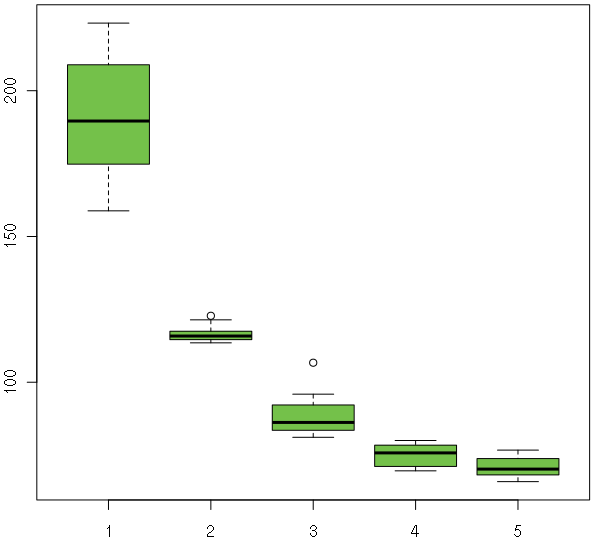
\includegraphics[scale=0.3]{images/execution_boxplot.png}
        \end{column}
        \begin{column}{.4\textwidth}
            \begin{center}
                \textbf{Box Plot}\\[0.3cm]
                10 ejecuciones por igual cantidad de clientes
            \end{center}
        \end{column}
    \end{columns}
\end{frame}

% \begin{frame}{Análisis de performance}
%     \begin{columns}[T]
%         \begin{column}{.5\textwidth}
%             \centering
%             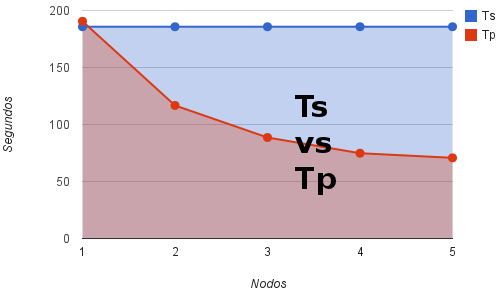
\includegraphics[scale=0.3]{images/ts_vs_tp.png}\\
%             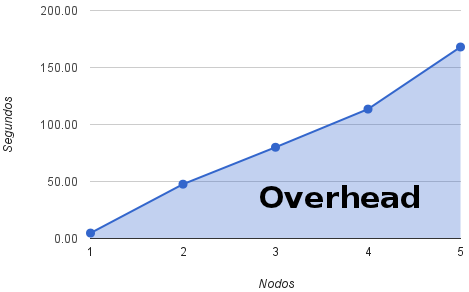
\includegraphics[scale=0.3]{images/overhead.png}
%         \end{column}
%         \begin{column}{.5\textwidth}
%             \centering
%             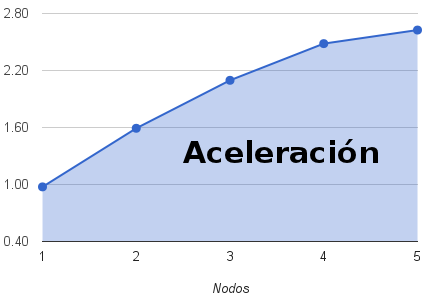
\includegraphics[scale=0.3]{images/speedup.png}\\
%             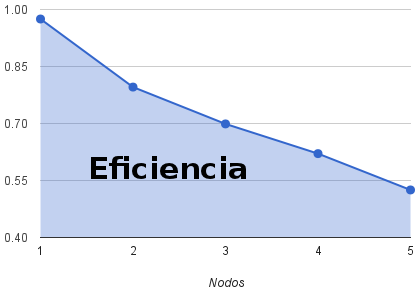
\includegraphics[scale=0.3]{images/eficiency.png}
%         \end{column}
%     \end{columns}
% \end{frame}


\begin{frame}\frametitle{CombEng}
        % montada sobre \rc\ y por consecuencia sobre \fud\
        Es una nueva capa  que engloba la familia de problemas cuya soluciones involucran un motor combinatorio.

        \begin{block}{Características}
            \begin{itemize}
                \item Provee un motor combinatorio para la generación de árboles de combinaciones.
                \item Utiliza mecanismos de poda sobre dichos árboles.
                \item Posee un sistema de puntuación por cada una de las combinaciones (\textit{ranking} o \textit{scoring}).
            \end{itemize}         
        \end{block}
         
\end{frame}

\begin{frame}\frametitle{CombEng}
        En resumen:
        \begin{center}
            \only<1>{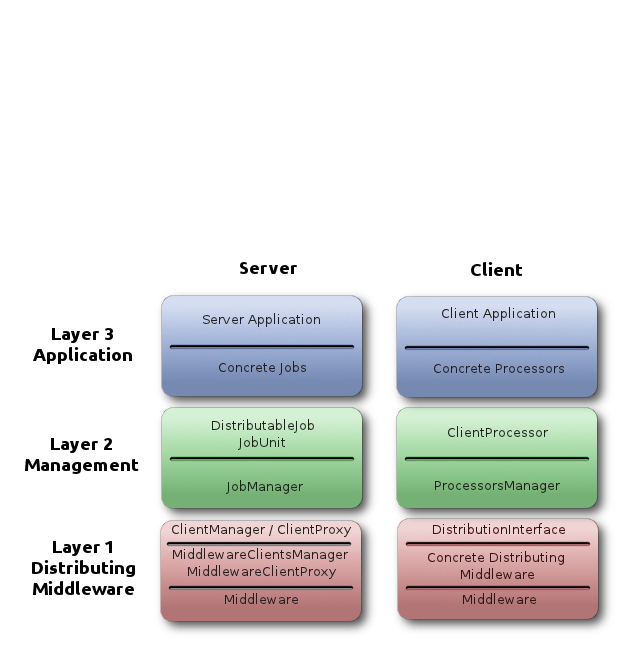
\includegraphics[scale=.3]{images/fud-l2.png}}
            \only<2>{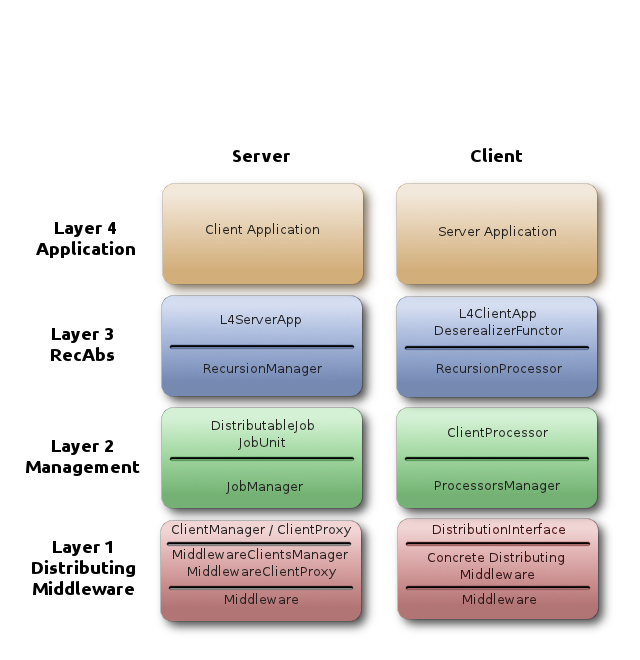
\includegraphics[scale=.3]{images/fud-l3.png}}
            \only<3>{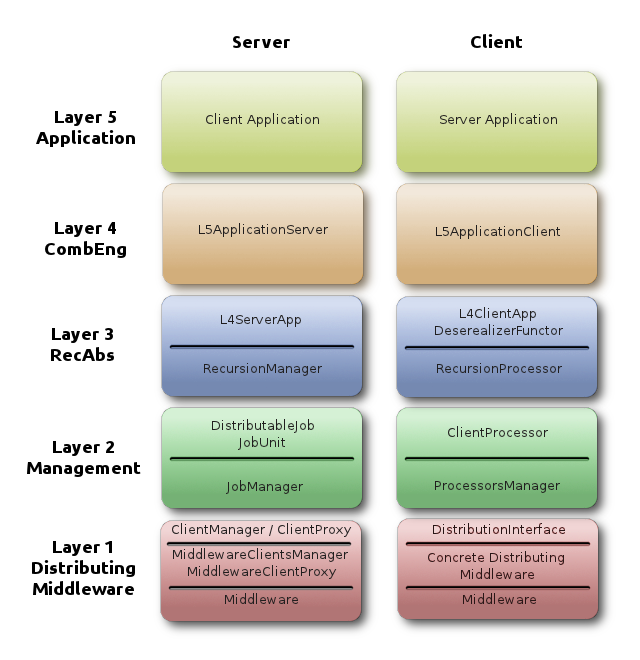
\includegraphics[scale=.3]{images/fud-l4.png}}
        \end{center}
\end{frame}

\begin{frame}\frametitle{RNAFoldingFreeEnergy}
    \textbf{HIV y los Antirretroviral}
    \begin{itemize}
     \item Un infectado con VIH es sometido a una intensiva terapia antirretroviral.
     \item Una terapia es la suceción de aplicaciones de antirretrovirales en el tiempo
     \item En cada paso se le suministra al paciente una combinación de uno o más antirretrovirales
     \item Cuando a una persona se le aplica un antirretroviral, el virus comienza a mutar hasta que logra hacerse resistente. 
    \end{itemize}


% El orden en que se aplican los antirretrovirales y cómo éstos son combinados, son factores muy importantes que determinan, entre otras
% cosas, el tiempo que transcurre hasta el momento en que el virus sea resistente a todos los antirretrovirales.

\begin{block}{RNAFFE}
    Recopila informaci\'on sobre como var\'ia la Energ\'ia Libre en la estructura secundaria del RNA viral a medida que los
    antirretrovirales son aplicados sobre la persona infectada.
\end{block}

\end{frame}

\begin{frame}\frametitle{RNAFoldingFreeEnergy}
    \begin{center}
        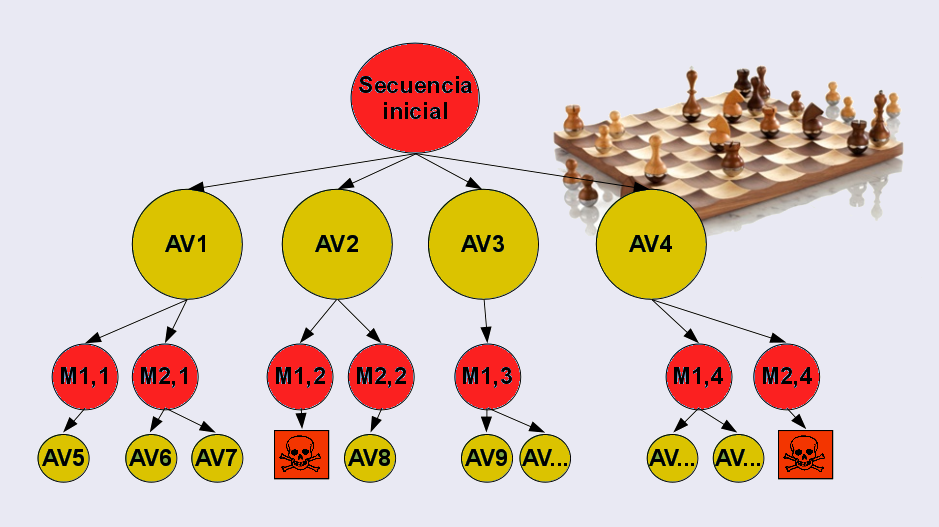
\includegraphics[width=\linewidth]{images/Arbol_ajedrez.png}
    \end{center}
\end{frame}
\section{Refactorización de FuD}

\begin{frame}{Refactorización de FuD}
%     \begin{block}{}\centering \rc{} $+$ \fud{} $\neq$ articulación 100\%\end{block}

        \centering
        \only<1-3>{
\includegraphics[scale=0.4]{images/fud-recabs-non-compatible.png}}
%             \centering
        \only<4>{
\includegraphics[scale=0.4]{images/fud-recabs-compatible.png}}

    \vspace{0.5cm}
    \pause
    \begin{center}
        \begin{Large}¿Qué faltaba en \fud{}?\end{Large}
        \vspace{0.7cm}
        \pause
        \begin{itemize}
            \item  Envío de mensajes de cliente a servidor.\\ \rc: \textit{envío de resultados y trabajos en cualquier momento}.
            \vspace{0.2cm}
            \pause
            \item  Pedido y reserva de clientes.\\ \rc: \textit{balanceo de carga dinámico con respecto a disponibilidad de clientes}.
        \end{itemize}

    \end{center}

\end{frame}


\subsection{Diseño}

\begin{frame}{Diagrama de clases}
    \only<1>{
        \centering
            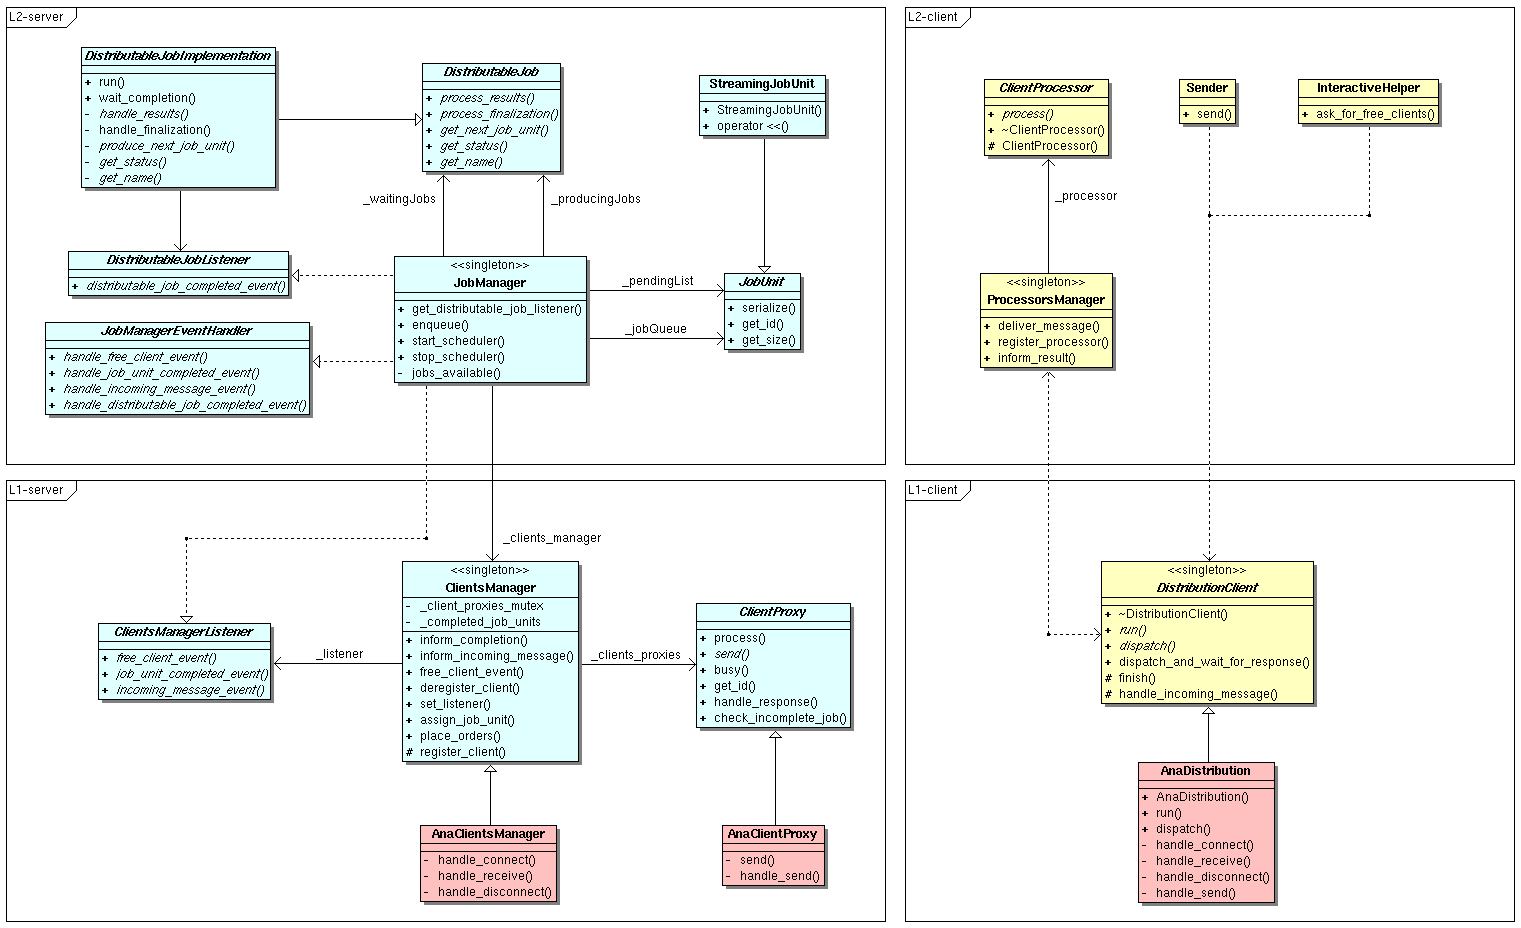
\includegraphics[scale=0.21]{images/fud_class.png}
    }
    
    \only<2>{
        \begin{center}
            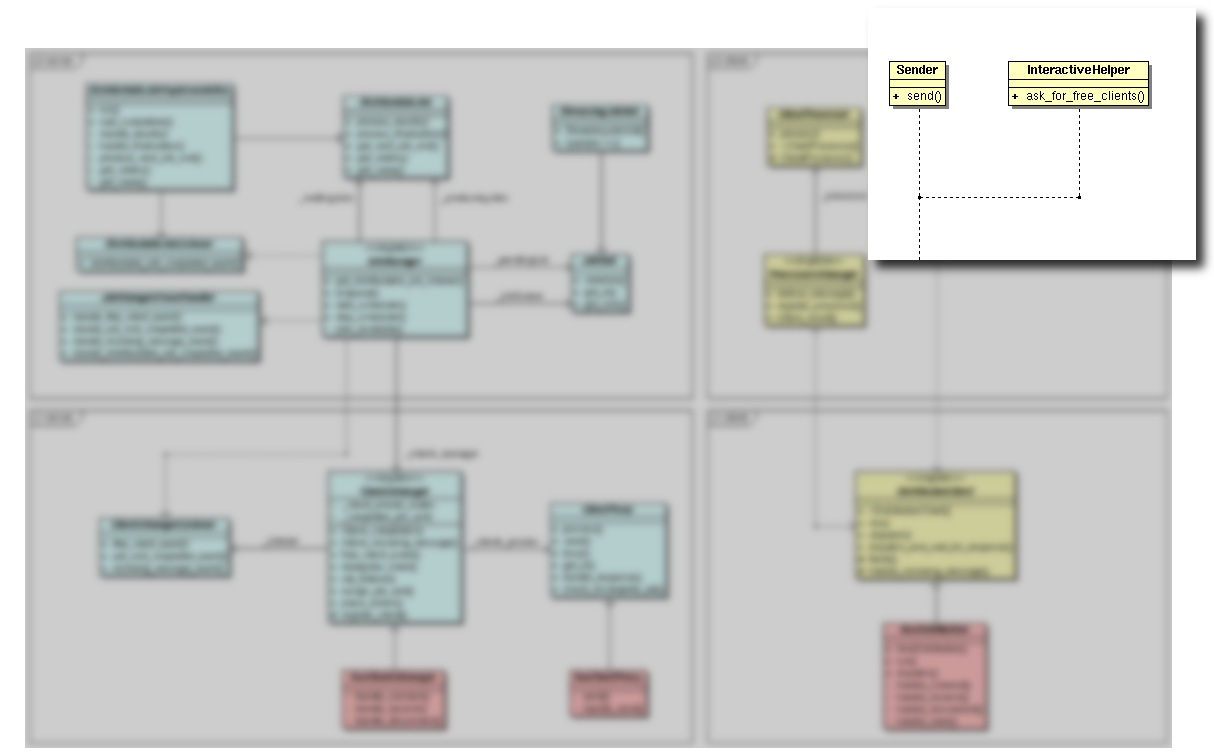
\includegraphics[scale=0.21]{images/fud_class-zoom.png}
        \end{center}
    }

\end{frame}

\begin{frame}{Lado Cliente: Antes}
    \begin{columns}[T]
        \begin{column}{.6\textwidth}
            \centering
            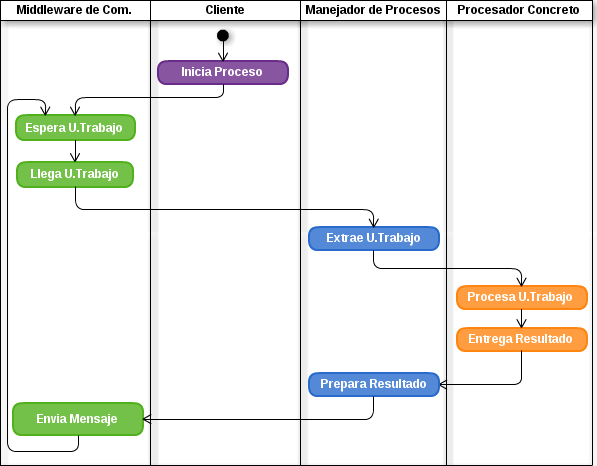
\includegraphics[scale=0.3]{images/ActivityFuDClient-Orig.png}
        \end{column}
        \begin{column}{.4\textwidth}
            \begin{enumerate}
                \item   Cliente recibe trabajo y lo procesa.
                \vspace{0.2cm}
                \item   Finalización del trabajo con envío de resultado final.
            \end{enumerate}
        \end{column}
    \end{columns}
\end{frame}

\begin{frame}{Lado Cliente: Después}
    \begin{columns}[T]
        \begin{column}{.6\textwidth}
            \centering
            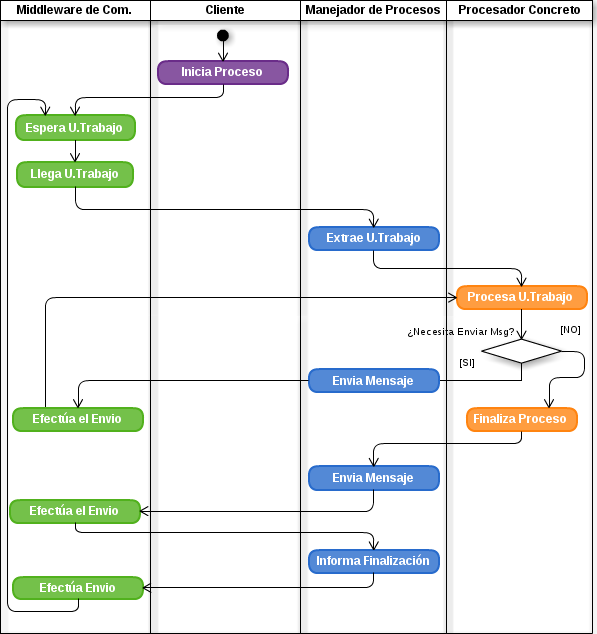
\includegraphics[scale=0.3]{images/ActivityFuDClient-Duplex.png}
        \end{column}
        \begin{column}{.4\textwidth}
            \begin{enumerate}
                \item   Cliente recibe trabajo, y empieza a procesar.
                \vspace{0.2cm}
                \item   Opción de enviar mensajes y/o trabajos no procesados.
                \vspace{0.2cm}
                \item   Finalización.
            \end{enumerate}
        \end{column}
    \end{columns}
\end{frame}

\begin{frame}{Lado Servidor: Antes}
    \begin{columns}[T]
        \begin{column}{.55\textwidth}
            \centering
            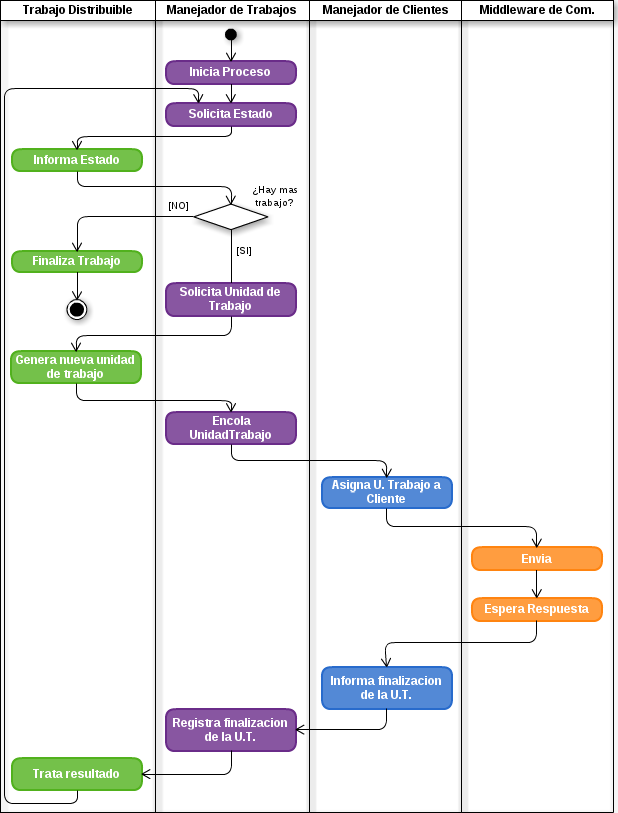
\includegraphics[scale=0.23]{images/ActivityFuDServer-Orig.png}
        \end{column}
        \begin{column}{.45\textwidth}
            \begin{enumerate}
                \item   Verifica si hay trabajos pendientes
                \vspace{0.2cm}
                \item   Genera unidad de trabajo (U.T.)
                \vspace{0.2cm}
                \item   Asigna U.T. a cliente libre
                \vspace{0.2cm}
                \item   Espera resultado final
                \vspace{0.2cm}
                \item   Finalización de U.T.
            \end{enumerate}
        \end{column}
    \end{columns}
\end{frame}

\begin{frame}{Lado Servidor: Después}
    \begin{columns}[T]
        \begin{column}{.55\textwidth}
            \centering
            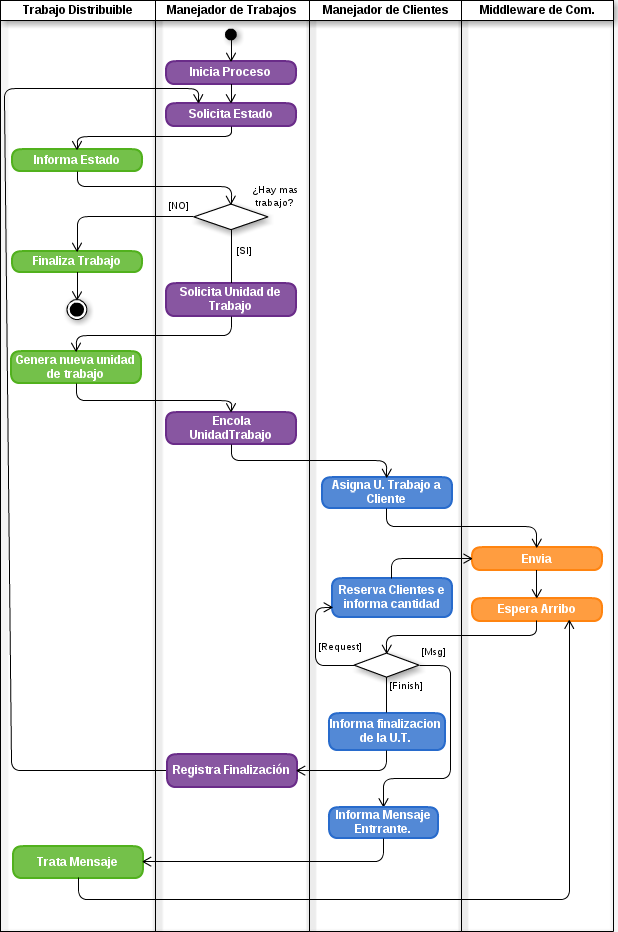
\includegraphics[scale=0.2]{images/ActivityFuDServer-Duplex.png}
        \end{column}
        \begin{column}{.45\textwidth}
            \begin{enumerate}
                \item   Verifica si hay trabajos pendientes
                \vspace{0.2cm}
                \item   Genera unidad de trabajo (U.T.)
                \vspace{0.2cm}
                \item   Asigna U.T. a cliente libre
                \vspace{0.2cm}
                \item   Espera mensaje, requerimiento de clientes libres o finalización de U.T.
                \vspace{0.2cm}
                \item   Trata mensaje correspondiente
                \vspace{0.2cm}
                \item   Finalización de U.T.
            \end{enumerate}
        \end{column}
    \end{columns}
\end{frame}


\subsection{Implementación}

\begin{frame}{Dependencias}
    La refactorización de \fud{} incluyó las siguientes librerías:
    \begin{description}
        \item[MiLi]: colección sencilla de pequeñas librerías útiles.
        \item[ANA]: librería de red asincrónica.
    \end{description}
\end{frame}

\begin{frame}{Métricas}
    La refactorización de \fud{} implicó la modificación de 21 archivos y la creación de 5 archivos, con un total de 1114 líneas de texto.
    \begin{center}
        \rowcolors{2}{verde!20}{verde!5}
        \begin{tabular}{|l|r|r|r|r|r|c|}
            \hline
            \multicolumn{3}{|c|}{Files} & \multicolumn{3}{|c|}{Line Types} & \hspace{0.2cm}\% \\
            \hline
            \textbf{Type} & \textbf{Mod.} & \textbf{Cre.} & \textbf{Blank} & \textbf{Com.} & \textbf{Source} & \small{\textbf{Com./Tot.}}\\
            \hline
            \texttt{C++ source} & 9   & 3   &    60  &    176   &   287 & 38.01 \\
            \hline
            \texttt{C++ header} & 12  & 2   &    88  &    403   &   100 & 80.11 \\
            \hline
            \textbf{Total}      & 21  & 5   &   148  & \color{blue}579\color{black} & \color{blue}387\color{black} & \textbf{59.93} \\
            \hline
        \end{tabular}
    \end{center}
\end{frame}
\section{Conclusión y trabajo futuro}

\begin{frame}{Herramientas}
%Herramientas utilizadas en \textit{FuDePAN}:\\[0.3cm]
\begin{itemize}
\item Google Code (svn, issue tracking, reviews, wiki, etc.).
\item Toolchain de GNU.
\begin{itemize}
    \item g++
    \begin{itemize}
    \item -Wall
    \item -pedantic
    \item -ansi
    \item -Weffc++
    \end{itemize}
    \item gdb
    \item gcov
\end{itemize}
\item CCCC
\item CLOC
\item gprof (GNU Profiler).
\item Valgrind
\item astyle (Artistic Style).
\item Doxygen
\item CMake
\end{itemize}

\end{frame}


\subsection{Conclusión}

\begin{frame}{Conclusión}

    \begin{itemize}
     \item \rc\ funciona correctamente, independientemente del problema a resolver
     \item Nueva version de \fud\ funcional compatible hacia atrás que funciona con la misma eficacia que antes.
     \item Se abordaron técnicas y conceptos no vistos a lo largo de la carrera.
     \item Se obtuvo un experiencia de desarrolo satisfactoria trabajando en conjunto con otros grupos, local y remotamente.
    \end{itemize}

\end{frame}


\subsection{Trabajo futuro}

\begin{frame}{Trabajo futuro}

    \begin{itemize}
        \item Proveer de nuevas políticas de distribución concretas.
        \item Adaptar esta capa para que proyectos \textbf{\textit{BOINC}} funcionen sobre ella.
        \item Correr \textit{\textbf{RNAFEE}} en ``modo completo'' en un cluster
        \item Reimplementar sobre \rc\ el generador de cadenas de proteínas \textit{backbones-generator}
    \end{itemize}
\end{frame}


\begin{frame}{Backbones Generator}
    
    Es un proyecto que tiene como objetivo construir una base de datos de las posibles cadenas principales (backbones) de
    proteínas.\\[0.5cm]
    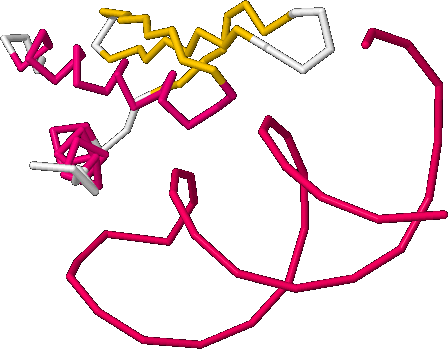
\includegraphics[height=120pt]{images/2L3C-backbone.png} 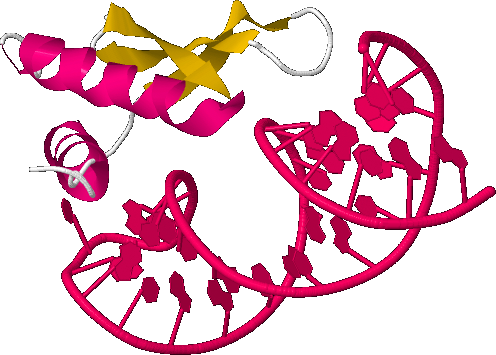
\includegraphics[height=120pt]{images/2L3C-cartoon.png}\\[0.2cm]
    \qquad \qquad \qquad \textit{backbone} \qquad \qquad \qquad \qquad \qquad \textit{proteína específica}
\end{frame}

\begin{frame}{Backbones Generator}
    \textit{Características:}
    \begin{itemize}
        \item Una predicción de una proteína puede durar varios meses.
        \item Una proteína tiene dos partes: cadena principal y cadenas laterales que la diferencian.
    \end{itemize}
    \begin{center}
        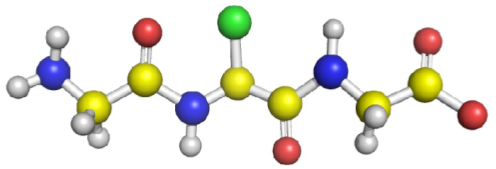
\includegraphics[height=40pt]{images/backbone.png}
    \end{center}
    \pause
    \begin{block}{Idea}
        Hacer por \textbf{única vez} un cálculo gigante que arroje una base de datos de todos los esqueletos de proteínas posibles de
        tamaño máximo dado.
    \end{block}
\end{frame}


%%%%%%%%%%%%%%%% BIBLIOGRAFIA %%%%%%%%%%%%%%%%
\nocite{alsuwaiyel98}
\nocite{bellman10}
\nocite{clus09}
\nocite{uml}
\nocite{buyya99}
\nocite{cormen09}
\nocite{ewd1036}
\nocite{algorithms06}
\nocite{flynn}
\nocite{parallel}
\nocite{conmath94}
\nocite{levitin06}
\nocite{Liskov:1987:KAD:62139.62141}
\nocite{Lorin:1990:RHP:1011116.1011127}
\nocite{objmentor}
\nocite{martin-asd}
\nocite{oosc}
\nocite{pressman}
\nocite{svn}
\nocite{sigler03}
\nocite{skiena08}
\nocite{moshe10}
\nocite{cplusplus}
\nocite{algdatpro76}

\begin{frame}[allowframebreaks]{Bibliografía} 
    \bibliography{biblio}
    \bibliographystyle{annotate}
\end{frame}

%%%%%%%%%%%%%%%% PREGUNTAS %%%%%%%%%%%%%%%%
\begin{frame}
    \centerline{\Huge{\textbf{?`Preguntas?}}}
\end{frame}

%%%%%%%%%%%%%%%% GRACIAS %%%%%%%%%%%%%%%%
\begin{frame}
    \centerline{\Huge{\textbf{GRACIAS}}}
\end{frame}


\end{document}